\documentclass[a4paper]{article}

\usepackage[magyar]{babel}
\usepackage{t1enc} % magyar elválasztás
\usepackage[utf8]{inputenc}
\usepackage{amsmath}
\usepackage{graphicx}
\usepackage{amssymb}
\usepackage{amsthm}
\usepackage{tikz-cd}
\usepackage{mathrsfs}
\usepackage[colorinlistoftodos]{todonotes}
\usepackage{enumitem}
\usepackage{yfonts}
\usepackage{ dsfont }

%
\usepackage{hyperref}

% https://tex.stackexchange.com/questions/124953/syntax-highlighting-in-listings-for-c-that-it-looks-like-in-visual-studio
%\setmonofont{Consolas} %to be used with XeLaTeX or LuaLaTeX
\definecolor{bluekeywords}{rgb}{0,0,1}
\definecolor{greencomments}{rgb}{0,0.5,0}
\definecolor{redstrings}{rgb}{0.64,0.08,0.08}
\definecolor{xmlcomments}{rgb}{0.5,0.5,0.5}
\definecolor{types}{rgb}{0.17,0.57,0.68}

\usepackage{listings}
\lstset{language=[Sharp]C,
	captionpos=b,
	%numbers=left, %Nummerierung
	%numberstyle=\tiny, % kleine Zeilennummern
	frame=lines, % Oberhalb und unterhalb des Listings ist eine Linie
	showspaces=false,
	showtabs=false,
	breaklines=true,
	showstringspaces=false,
	breakatwhitespace=true,
	escapeinside={(*@}{@*)},
	commentstyle=\color{greencomments},
	morekeywords={partial, var, value, get, set},
	keywordstyle=\color{bluekeywords},
	stringstyle=\color{redstrings},
	basicstyle=\ttfamily\small,
}

% https://tex.stackexchange.com/questions/64839/how-to-change-listing-caption
\renewcommand{\lstlistingname}{Programkód}% Listing -> Programkód
%

\title{Kezdő C\# programozás szakkör jegyzet}

\author{Szkupien Péter}

\date{2019. október\footnote{Ez a jegyzet eredetileg Wordben készült, 2022. szeptemberében alakítottam át \LaTeX-alapúvá.}}
\newtheorem{thm}{Theorem}[section]
\newtheorem{lem}[thm]{Lemma}

\newtheorem{defn}[thm]{Definíció} %
\newtheorem{eg}[thm]{Példa} %
\newtheorem{ex}[thm]{Feladat} %
\newtheorem{so}[thm]{Megoldás} %
\newtheorem{conj}[thm]{Conjecture}
\newtheorem{cor}[thm]{Corollary}
\newtheorem{claim}[thm]{Claim}
\newtheorem{rmk}[thm]{Remark}

% https://tex.stackexchange.com/questions/62020/how-to-change-the-word-proof-in-the-proof-environment
%\renewcommand*{\proofname}{Solution}
\newenvironment{solution} {\begin{proof}[Megoldás]} {\end{proof}}

\newcommand{\ie}{\emph{i.e.} }
\newcommand{\cf}{\emph{cf.} }
\newcommand{\into}{\hookrightarrow}
\newcommand{\dirac}{\slashed{\partial}}
\newcommand{\R}{\mathbb{R}}
\newcommand{\C}{\mathbb{C}}
\newcommand{\Z}{\mathbb{Z}}
\newcommand{\N}{\mathbb{N}}
\newcommand{\Q}{\mathbb{Q}}
\newcommand{\LieT}{\mathfrak{t}}
\newcommand{\T}{\mathbb{T}}
\newcommand{\A}{\mathds{A}}

\begin{document}
\maketitle

\section{Jegyzet}
Ez a jegyzet a Szent István Gimnázium 2019/2020-as kezdő C\# szakköréhez készült oktatási segédletként, nyelvezete és precizitása a szakkör hetedikes hallgatóságához igazodik (vagy legalábbis kíván igazodni). Ha elírást vagy hibát találsz benne, megköszönöm, ha jelzed a \href{mailto:peti.szkupien@gmail.com}{peti.szkupien@gmail.com} email címen vagy akár \href{https://github.com/szkupienpeti/csharp-lecture-notes/issues}{GitHub issue} formájában. Ha valamit nem értenél akár a jegyzetből, akár egy otthoni próbálkozás eredményéből, nyugodtan írj egy emailt, és szívesen válaszolok.

\section{Program, programozás madártávlatból}
Ha nagyon nagy vonalakban tekintünk a számítógépre és a rajta futó programokra, lényegében ugyanúgy működnek, mint bármilyen más kommunikáció is: vagy a felhasználó „mond valamit” a számítógépnek, vagy a számítógép „mond valamit” a felhasználónak. A programjaink, amiket írni fogunk, ezt a két dolgot fogják összekötni: lényegében azt a logikát fogjuk megvalósítani, ami összeköti a felhasználó és a számítógép tevékenységeit. (Pl.: a felhasználó beírja, hogy 2+2, a program kiírja, hogy 4. A kettő közti logika az, ami a programunk lényegét adja: értelmezni, hogy kettő számot és egy műveleti jelet kaptunk, rájönni, hogy az milyen művelet, elvégezni a műveletet, majd kiírni az eredményt. Ugye, hogy nem is olyan egyszerű?)

\section{Konzol}
A fent leírt kommunikációt egy egyszerű konzolon keresztül fogjuk megvalósítani. Természetesen vannak csili-vili felületek is, ahol szép rózsaszín gombokat gyárthatunk, de ezek ugyan szépek, de cserébe talán el is terelik a figyelmet a lényegről. A konzol, amit használni fogunk, egy nagyon egyszerű fekete hátterű ablak, amire fehér karakterek írhatók. Vagy a programunk ír ki rá valamit a felhasználónak, vagy a felhasználó ír be valamit a programnak. Ennyire egyszerű.

\section{Visual Studio, C\#}
A Microsoft \textbf{Visual Studio} nevű fejlesztőkörnyezetében fogunk programozni, C\# nyelven. A Visual Studio egy rendkívül összetett fejlesztőeszköz, aminek mi értelemszerűen csak néhány nagyon alapvető funkcióját fogjuk használni. A \textbf{C\#} (\emph{ejtsd: szí sárp}) egy magasszintű programozási nyelv, vagyis olvasható kódot írhatunk benne, viszonylag könnyen.

A Visual Studio az iskolai gépekre fel van telepítve, de otthon is elérhető ingyenesen: a Visual Studio Community 2019 letölthető a \href{https://visualstudio.microsoft.com/}{visualstudio.com} oldalról, a használatához csak be kell jelentkezni egy tetszőleges Microsoft-fiókba (ez lehet akár az iskolai is, akár egy „privát” is).

\section{Projekt}
A Visual Studio-ban írt programjaink projektekbe rendeződnek, vagyis, ha új programot szeretnénk írni, új projektet kell létrehoznunk (\emph{természetesen egy projektben több fájl is lehet, de ennek a hogyanjának a megértéséhez olyan ismeretekre lenne szükség, amelyeknek egyelőre nem vagyunk birtokában, így fogadjuk el az ökölszabályt, hogy mindig új projektet hozunk létre}).

Új projektet a New project menüponttal hozhatunk létre (ennek a menüpontnak a helye függ a konkrét Visual Studio-verziótól, de az indításkor megjelenő képernyőn mindig könnyen megtalálható). Válasszuk a C\# nyelvű Console Application (.NET Framework) projekttípust. Ezután megadható a projekt neve, valamint a mappa, ahová menteni szeretnénk (általánosságban elmondható, hogy érdemes az elérési utakban és nevekben tartózkodni az ékezetektől, szóközöktől, különleges karakterektől stb.)

\emph{A kiválasztott helyre létrejött projektünk sok fájlt tartalmaz, amelyekre általában nekünk nincs szükségünk, de a Visual Studionak fontosok, így természetesen nem szabad kitörölni őket. Ha a programkódunkat keressük, a projektmappában a projekt neve/Program.cs fájlban találjuk, a futtatható .exe fájl pedig a projekt neve/bin/Debug helyen jön létre (az első fordításkor).}

Ha létrejött a projektünk, megismerkedhetünk a Visual Studio felépítésével. A funkciók nagy részére nincs szükségünk, a legfontosabbak:

\begin{itemize}
	\item \textbf{Solution Explorer}, általában az ablak jobb szélén: itt találjuk a projektünk felépítését, innen tudjuk megnyitni a Program.cs fájlt, amelyikbe a programkódot írjuk, ha véletlenül bezárnánk. Ha nem látjuk a Solution Explorert, a View/Solution Explorer menüponttal megjeleníthetjük.
	\item \textbf{Programkód}, középen: itt szerkeszthetjük a programunk kódját.
	\item \textbf{Error List}, általában az ablak alján: itt olvashatjuk a programunkban lévő (szintaktikai) hibákat, amennyiben vannak ilyenek. Ezek angol nyelvű hibaüzenetek, de nagyon hasznos, ha valaki tudja őket értelmezni. Ha nem látjuk az Error Listet, a View/Error List menüponttal megjeleníthetjük.
\end{itemize}

A programunkat az F5 gombbal, vagy az eszköztáron található zöld színű nyíllal jelzett Start gombbal indíthatjuk el.

\section{Hello World!}
A létrejött Program.cs fájlunk egyáltalán nem üres, elsőre sok furcsa karaktersorozatot találunk benne. A jó hír, hogy ezekkel többnyire egyelőre semmi dolgunk nem lesz, korán vagyunk még ahhoz, hogy megértsük, mi mit jelent. Alapértelmezetten ezt kell látnunk:

\begin{lstlisting}[caption=Hello World!, label=lst:hello]
using System;
using System.Collections.Generic;
using System.Linq;
using System.Text;
using System.Threading.Tasks;

namespace ConsoleApp1
{
  class Program
  {
    static void Main(string[] args)
    {
    }
  }
}
\end{lstlisting}

Amit talán érdemes megjegyeznünk, hogy a \lstinline{static void Main} kezdetű sor a programunk \emph{belépési pontja}, vagyis itt fog elkezdeni igazából futni. Az ezt a sort követű \lstinline!{ }!-ba (kapcsoszárójelpár, blokk) fogjuk írni egyelőre a teljes programkódunkat. Ennek megfelelően a további példa programkódoknál nem írjuk le mindig ezt a teljes „körítést”, csak a \lstinline{Main}-en belüli részre szorítkozunk.

Hagyományosan minden programozást oktató könyv/kurzus egy olyan programmal kezdődik, ami kiírja, hogy ”Hello World!”, így mi is ezzel kezdünk. A korábban már említett konzolra a \lstinline{Console.WriteLine("HelloWorld!");} sorral tudjuk ezt kiírni.

Figyeljük meg ezt az egyszerű sort! A \lstinline{Console} az a \emph{valami}, amit használni szeretnénk, a \lstinline{WriteLine} az a \emph{valami}, amit csinálni szeretnénk a konzollal, a kettő között pedig egy pont áll. Az elnevezések angolok, nagybetűvel kezdődnek, a többszavas nevekben pedig a szóhatárt szintén nagybetűvel jelöljük. A \lstinline{WriteLine}-t egy zárójelpár követi, amiben idézőjelek között áll a kiírandó szöveg. A sort egy pontosvessző zárja.

Nagyon nem precíz, de egyelőre praktikus ökölszabályként elmondható, hogy azokat a nevesített utasításokat, amik \emph{valamivel csinálnak valamit} zárójelpár követi, amiben (amennyiben vannak) megadhatjuk azokat a részleteket, amik pontosítják, hogy mi fog történni. Ebben az esetben az utasítás, ami \emph{valamivel csinál valamit} a \lstinline{WriteLine}, hiszen kiír valamit a konzolra. A zárójelpárban pedig megadhatjuk, hogy mit írjon ki, ez lényegében pontosítja a működést. (\emph{Szakkifejezéssel élve a \lstinline{WriteLine}-t függvénynek vagy metódusnak, a zárójelpárban lévő dolgokat pedig paramétereknek nevezzük.}) A kiírandó szöveget idézőjelek közé írjuk, ezzel jelezzük a számítógépnek, hogy ez egy sima szöveg, nem pedig egy utasítás. Minden utasítás sor végére pontosvesszőt teszünk. (Alt Gr+?)

\emph{Ha nem azt szeretnénk kiírni, hogy HelloWorld!, csak egy üres sort, a zárójelpárt üresen hagyhatjuk, de akkor sem hagyhatjuk el.}

\subsection{Nem működik a program?!}
Ha a fenti Hello Worl\d! programot lefuttatjuk, valószínűleg nem fogjuk látni a hőn áhított eredményt, legfeljebb egy pillanatra felugró, majd rögtön el is tűnő fekete ablakot. Ennek az az oka, hogy a programunk sorra hajtja végre az utasításokat, majd, ha a végére ért, egyszerűen leáll. Ez történik itt is, olyan gyorsan írja ki ezt az egy sort, majd áll is le rögtön, hogy mi azt észre sem vesszük. Ha szeretnénk megbizonyosodni róla, hogy valóban kiírtuk, amit akartunk, tegyük a programunk legvégére a következő sort:

\begin{lstlisting}[caption=Várakozás billentyűleütésre, label=lst:readkey]
Console.ReadKey();
\end{lstlisting}

Ennek hatására a programunk a végén várni fog tőlünk egy billentyűleütést, és csak utána fog bezáródni. Azt, hogy ez pontosan mit jelent, a későbbiekben tárgyaljuk.

\subsection{Megjegyzések}
A programkódunkba írhatunk megjegyzéseket, amiket a számítógép figyelmen kívül hagy, de magunknak hasznosak lehetnek, átláthatóbbá tehetik a programkódunkat. Egysoros megjegyzést \lstinline{//} után írhatunk, több sorost pedig a \lstinline{/* ... */} közé.

\begin{lstlisting}[caption=Megjegyzések, label=lst:comments]
// ez egy megjegyzes, barmit irhatunk ide, nem szamit
/* ez egy tobb soros megjegyzes
egeszen addig, amig
le nem zarjuk */
\end{lstlisting}

\section{Változók}
A programjaink persze nem sokat érnének, ha mindent előre beléjük kellene írnunk. Adja magát az igény, hogy valahogy el tudjunk tárolni értékeket, és azokat utána (újra) fel tudjuk használni. Például, ha a programunk egyszerűen megszorozza kettővel a kapott számokat, akkor is először el kell tárolnunk a beírt számot, hogy utána meg tudjuk szorozni kettővel.

Képzeljük el ezt úgy, mintha lennének dobozaink, amikbe be tudunk tenni dolgokat, később pedig meg tudjuk nézni, mi van bennük, és le is tudjuk cserélni a tartalmukat. A dobozaink viszont különböző formájúak, és mindegyikbe csak olyan formájú dolgot tehetünk, amilyen a doboz.

\begin{figure}[h!]
	\centering
	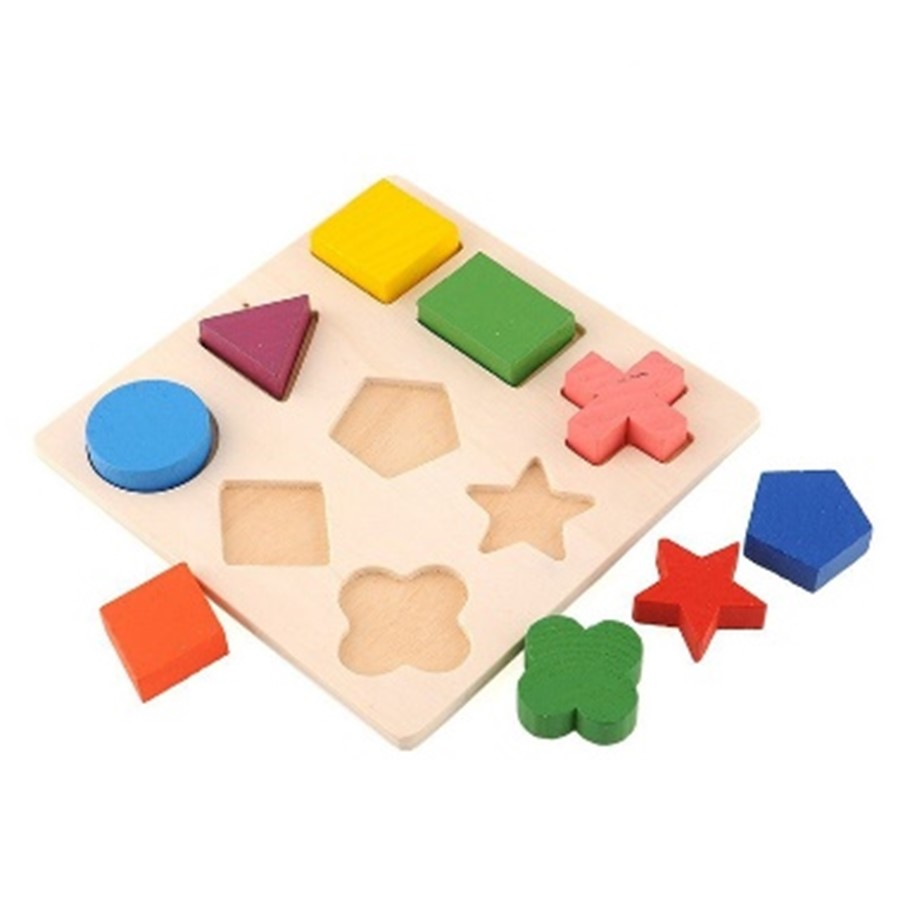
\includegraphics[width=3cm]{figures/variables.jpg}
\end{figure}

A dobozainkat használni is szeretnénk később, így megkülönböztethetők kellenek, hogy legyenek. Mindegyiknek kell, hogy legyen tehát egy egyedi neve, ami beazonosítja.

A fenti mondatok lényegében meg is határozták, mit értünk változó alatt: egy típussal és egyedi névvel rendelkező valami, ami típusának megfelelő értéket tud tárolni, amit ki tudunk olvasni és meg tudunk változtatni. (Innen ered a változó elnevezés: egy olyan logikai egység („doboz”), aminek az idő múlásával változhat az értéke.)

A változó típusa lényegében bármi lehet, a teljesség igénye nélkül a legelemibbek:
\begin{itemize}
	\item \textbf{egész szám} (\lstinline{int})
	\item \textbf{tört szám} (\lstinline{float}): programozásban az angol nyelvhez hasonlóan tizedespontot használunk, nem tizedesvesszőt
	\item \textbf{karakter} (\lstinline{char}): ez egyetlen karaktert jelent, ami persze nem csak betű lehet, hanem számjegy, írásjel, bármi. A karaktereket szimpla idézőjelbe tesszük, pl.: ’a’
	\item \textbf{szöveg} (\lstinline{string}): bármilyen hosszú lehet a szövegünk (vagyis akár üres is), amit (dupla) idézőjelbe teszünk, pl.: ”szöveg”, ”” (utóbbi az üres string)
	\item \textbf{logikai érték} (\lstinline{bool}): igaz (\lstinline{true}) vagy hamis (\lstinline{false})
\end{itemize}

Most, hogy tudjuk, mit jelent a változó, és milyen típusai lehetnek, már csak az a kérdés, hogyan használjuk őket a programkódunkban. Létrehozhatunk egy változót anélkül, hogy megadnánk a kezdeti értékét (természetesen valamilyen alapértelmezett értéke ekkor is lesz, csak azt nem mi adjuk meg explicit – szám esetén 0, logikai érték esetén a hamis az alapértelmezett érték, de mindig adjunk értéket a változóinknak, mielőtt használnánk őket!) és úgy is, hogy rögtön értéket is adunk neki (előbbit deklarációnak, utóbbit definíciónak hívjuk). Változót a típus és a változónév megadásával hozhatunk létre, a pontosvessző természetesen kell a sor végére.

\begin{lstlisting}[caption=Változók, label=lst:variables]
int szam = 5;    // szam nevu int tipusu valtozo, 5 ertekkel
string szoveg;   // szoveg nevu string tipusu valtozo
szoveg = "szia"; // kesobb adtunk erteket neki
\end{lstlisting}

\subsection{Értékadás és egyenlőségjel}
Fontos tisztázni, mit is jelent a programjainkban az egyenlőségjel. Nézzük például a következő kódot!

\begin{lstlisting}[caption=Értékadás, label=lst:assignment]
int szam = 5; // ez utan a sor utan szam erteke 5
szam = 10;    // ez utan a sor utan szam erteke 10
\end{lstlisting}

Az első sorban létrehoztunk egy \lstinline{szam} nevű, \lstinline{int} típusú változót, aminek 5-öt adtunk értékül. A második sor viszont már érdekesebb: az egyenlőségjel bal oldalán egy 5 értékű változó áll, a jobb oldalon pedig a 10. Jól jegyezzük meg, ez nem azt jelenti, hogy ez a két dolog egyenlő ($5 \neq 10$), hanem hogy a \lstinline{szam} nevű változónak értékül adjuk a 10-et. Az egyenlőségjel tehát programozásban az értékadás jele, nem pedig az egyenlőségvizsgálaté (arról, hogy utóbbinak akkor mi a jele, hamarosan).

\emph{Ne felejtsük el, hogy a változóneveknek egyedieknek kell lenniük! A fenti példák külön-külön értelmezendők, ezt az öt sort egymás után leírva hibás programot kapnánk, hiszen kétszer hozunk létre \lstinline{szam} nevű változót.}

\section{Beolvasás}
Azt már tudjuk, hogyan tudunk kiírni a konzolra, azt viszont még nem, hogy hogyan tudunk onnan beolvasni a felhasználótól. Ezt nem véletlenül a változók után tárgyaljuk: a beolvasásnak akkor van értelme, ha el is tudjuk tárolni a beolvasott érétket, ezt pedig egy változóval tudjuk megtenni.

\begin{lstlisting}[caption=Beolvasás, label=lst:read]
string szoveg = Console.ReadLine();
\end{lstlisting}

Így kell létrehozni egy \lstinline{szoveg} nevű, \lstinline{string} típusú változót, és beolvasni bele egy sort a konzolról. A \lstinline{ReadLine()} ugyanúgy metódus, mint a \lstinline{WriteLine()} volt, vagyis ennek a végére is zárójelpárt kell tennünk. A fenti példában tehát a \lstinline{Console.ReadLine()} beolvas egy sort a felhasználótól, majd ezt értékül adjuk a frissen létrehozott \lstinline{szoveg} nevű változónak.

\emph{A \lstinline{Console.ReadLine()} egy sort olvas be a felhasználótól, a sorokat pedig enterrel zárjuk. Vagyis egy \lstinline{ReadLine}-os programsor mindig vár egy entert, másképp fogalmazva a programunk egészen addig nem megy tovább, amíg a felhasználó entert nem üt.}

Most már van elég tudásunk ahhoz, hogy megértsük, miért írtunk a programjaink végére \lstinline{Console.ReadKey();}-t. A \lstinline{Console.ReadKey()} ugyanúgy vár egy billentyűleütést, ahogy a \lstinline{Console.ReadLine()} egy entert a sor végén. A különbség csak annyi, hogy míg a \lstinline{ReadLine} által beolvasott sort eltároljuk egy változóba, a \lstinline{ReadKey}-t nem erre használtuk, hanem csak arra, hogy várjon a programunk egy billentyűleütésig. (Egyébként a \lstinline{ReadKey}-jel beolvasott valamit is el lehetne tárolni, de ennek a típusa és a működése meghaladja jelenlegi tudásunkat.)

Az előző példában szöveget olvastunk be a konzolról, amit eltároltunk egy szöveg típusú változóba. Ha azonban számot szeretnénk beolvasni, egy kicsit nehezebb dolgunk van. A következő sor ugyanis NEM működik, hiába írná be a felhasználó a konzolra, hogy 123.

\begin{lstlisting}[caption=Hibás beolvasás, label=lst:readWrong]
int szam = Console.ReadLine(); //ez NEM mukodik
\end{lstlisting}

A problémát az okozza, hogy a \lstinline{ReadLine()} egy szöveget (\lstinline{string}-et) olvas be a konzolról, az \lstinline{int} típusú változóba pedig nem tehetünk \lstinline{string}-et (emlékezzünk vissza: a kör alakú dobozba nem passzol a négyzet). A beolvasott szövegből tehát valahogyan számot kell „csinálnunk”.

\begin{lstlisting}[caption=Egész szám beolvasása, label=lst:readIntParse]
int szam = int.Parse(Console.ReadLine());
\end{lstlisting}


Erre szolgál az \lstinline{int.Parse()}, ami a „hasába betett” szövegből \lstinline{int}-et csinál (szebben mondva: az \emph{argumentumként} kapott \lstinline{string}-et \lstinline{int}-té konvertálja). Ezt ugyanígy megtehetjük törtek esetében is, csak \lstinline{int} helyett \lstinline{float}-ot kell írnunk:

\begin{lstlisting}[caption=Törtszám beolvasása, label=lst:readFloatParse]
float tort = float.Parse(Console.ReadKey());
\end{lstlisting}

Azt már tudjuk, hogy programkódban a törtekben tizedespontot használunk, de beolvasásnál ez egy kicsit bonyolultabb. Az, hogy vesszőt vagy pontot kell-e használnunk, az operációs rendszerünk területi beállításaitól függ (magyar Windows esetén vessző, angol esetén pont).

\section{Változók értékének kiírása}
Azt már láttuk, hogyan írhatunk ki egy általunk beírt szöveget a konzolra, ez azonban önmagában nem túl hasznos. A programunknak pont az a lényege, hogy reagálni tud a felhasználó bemeneteire, vagyis nyilvánvalóan nem tudjuk (és nem is akarjuk) előre beírni az összes szöveget, amit majd valaha ki szeretnénk írni. Adja magát tehát az igény, hogy a konzolon megjelenő szövegbe változók értékeit is belefűzzük. Ezt többféle módon is megtehetjük, a példákban beolvasunk két számot, és összeadjuk őket, majd kiírjuk az eredményt „a és b összege c” alakban.

\subsection{Egy nem javasolt módszer}
Az elsőre legegyszerűbbnek tűnő módszer többnyire ugyan működik, de nagyon nem elegáns és könnyű elhibázni. Az alapja, hogy a szövegeket \lstinline{+} jellel össze tudjuk adni, így a \lstinline{Console.WriteLine()} zárójelpárjában az idézőjelek közt lévő szövegek és a változónevek közé egyszerűen \lstinline{+} jelet teszünk.

\begin{lstlisting}[caption=Változók értékének kiírása -- nem elegánsan, label=lst:writeVarsNotElegant]
int a = int.Parse(Console.ReadLine()); // 1
int b = int.Parse(Console.ReadLine()); // 2
int ossz = a + b;                      // 3
Console.WriteLine(a + " es " + b + " osszege " + ossz);
// 1 es 2 osszege 3
\end{lstlisting}

\subsubsection{A probléma}
A fenti módszerrel van azonban egy probléma, amibe könnyen beleszaladhatunk. A \lstinline{+} jel nem mindig azt csinálja, amit várnánk tőle. A fenti kódot egy kicsit másképp írva elsőre meglepő eredményt kapunk.

\begin{lstlisting}[caption=Változók értékének kiírása -- hibásan, label=lst:writeVarsError]
int a = int.Parse(Console.ReadLine()); // 1
int b = int.Parse(Console.ReadLine()); // 2
Console.WriteLine(a + " es " + b + " osszege " + a+b);
// 1 es 2 osszege 12
\end{lstlisting}

A fenti kód ugyan lefut, de elsőre azt hihetnénk, elromlott a számítógép, hiszen a konzolon a következő jelenik meg: \lstinline{1 es 2 osszege 12}

Ennek az oka, hogy a \lstinline{Console.WriteLine()} zárójelpárjában a számítógép balról jobbra haladva elkezdi elvégezni a műveleteket, de mivel a \lstinline{+} jel egyik oldalán szám, a másik oldalán pedig szöveg áll, azokat szövegként fűzi össze, nem pedig számként adja össze. Persze ha az \lstinline{(a+b)}-t zárójelbe tesszük, már működik, de ezt nagyon könnyű elfelejteni, és a programunk még csak nem is fog nekünk szólni, hogy elrontottunk valamit, egyszerűen csak (számunkra) butaságot fog kiírni.

Kezdőként elég nehéz mindig átlátni, hogy az ilyen műveletek esetén pontosan mi történik, és egyéb mélyebb okai is vannak, hogy nem célszerű így összefűzni szövegeket. Röviden tehát annyit jegyezzük meg, hogy a fenti módszert NE használjuk.

\subsection{Az elegáns módszer}
\begin{lstlisting}[caption=Változók értékének kiírása -- elegánsan, label=lst:writeVarsElegant]
int a = int.Parse(Console.ReadLine()); // 1
int b = int.Parse(Console.ReadLine()); // 2
int ossz = a + b;                      // 3
Console.WriteLine("{0} es {1} osszege {2}", a, b, ossz);
//1 es 2 osszege 3
\end{lstlisting}

A \lstinline{Console.WriteLine()} zárójelpárjába, az idézőjelen belülre teszünk \lstinline!{n}! jelölőket (\lstinline!{0}!, \lstinline!{1}! stb.), amik helyére a később felsorolt változóink értéke fog behelyettesítődni. A \lstinline!{n}!-ben az \lstinline{n} egy sorszámot jelöl, azt a sorszámot, ami szerint a szöveg után, a zárójelpáron belül felsoroljuk vesszővel a változókat. Nagyon fontos, hogy ez a sorszámozás 0-val kezdődik, vagyis a fenti példában a \lstinline!{0}! az első felsorolt változó, vagyis az \lstinline{a}; a \lstinline!{1}! a második felsorolt változó, vagyis a \lstinline{b}; a \lstinline!{2}! pedig a harmadik felsorolt változó, vagyis az \lstinline{ossz}.

\subsection{Egy újabb elegáns módszer}
Az előző módszer szépséghibája, hogy ha hosszú a szövegünk, olvasás közben nagyon nehéz átlátni, mit is fog kiírni, hiszen a tekintetünknek folyamatosan ugrálnia kell a \lstinline!{n}! jelölők és a sor végén lévő változónevek között. Ezt valahogy úgy tudnánk megoldani, ha a sor vége helyett a szövegben magában helyeznénk el a változóneveket, de ezt „csak úgy simán” nyilván nem tehetjük meg, hiszen akkor sehonnan sem derülne ki, hogy az a betű egy névelő vagy egy változónév.

\begin{lstlisting}[caption=Változók értékének kiírása -- elegánsan 2., label=lst:writeVarsElegant2]
int a = int.Parse(Console.ReadLine()); // 1
int b = int.Parse(Console.ReadLine()); // 2
int ossz = a + b;                      // 3
Console.WriteLine($"{a} es {b} osszege {ossz}");
// 1 es 2 osszege 3
\end{lstlisting}

% https://github.com/jgm/pandoc/issues/1629
\newcommand{\within}[1]{#1}

Ha a szöveg idézőjele elé teszünk egy \within{\lstinline{\$}} jelet, akkor a \lstinline!{}! kapcsoszárójelpárokba sorszám helyett változónevet is írhatunk. Ekkor értelemszerűen nem kell a szöveg után felsorolni újra a változókat. Ez a jelölés elsőre bonyolultnak tűnhet a sok különleges karakter miatt (dollárjel, idézőjel, kapcsos zárójel), de összességében ez eredményezi a legolvashatóbb programkódot.

\section{Aritmetikai műveletek}
A matematikai alapműveletek természetesen használhatók a programkódokban is, így összeadni, kivonni, szorozni és osztani minden további nélkül tudunk.

\begin{lstlisting}[caption=Aritmetikai műveletek, label=lst:arithemtics]
int a = 3, b = 4;
// egy sorban tobb azonos tipusu valtozot is letrehozhatunk
int osszeg = a + b; // 7
osszeg = osszeg - 1;
// osszeg erteket 1-gyel csokkentettuk, vagyis 6 lett
int negyzet = osszeg * osszeg; // 36
\end{lstlisting}

\emph{Figyeljük meg az \lstinline{osszeg = osszeg - 1;} sort, és emlékezzünk vissza, hogy az egyenlőségjel nem egyenlőséget, hanem értékadást jelent!}

\subsection{Az osztás és a problémák}
Két egész szám összege, különbsége és szorzata is biztosan egész lesz, a hányadosuk azonban már egyáltalán nem biztosan, ez pedig okoz némi kellemetlenséget. Elsőre talán meglepő, de a legtöbb programozási nyelvben (a C\# is ilyen) két egész szám hányadosa is egész lesz. Vagyis például \lstinline{3 / 4} eredménye \lstinline{0} lesz. Ezt egészosztásnak hívjuk, vagyis az osztási maradékkal „nem foglalkozunk”, a hányadost lefelé kerekítjük.

\begin{lstlisting}[caption=Egészosztás, label=lst:intDiv]
int a = 3, b = 4;
Console.WriteLine(a / b); // 0
Console.WriteLine(3 / 4); // 0
\end{lstlisting}

Talán még másodikra is meglepő, de két egész szám hányadosa még akkor is egész lesz, ha egy \lstinline{float} típusú változóban tároljuk el a „hányadost”. (Valójában ez nem meglepő: értékadásnál először kiértékelődik az egyenlőségjel jobb oldalán található kifejezés, és utána kerül bele az eredmény a változóba. Vagyis az osztás elvégzésekor a számítógép még nem tudja, mit fogunk csinálni az eredménnyel, kiírjuk a konzolra vagy értékül adjuk egy változónak.)

\begin{lstlisting}[caption=Egészosztás tört változóval, label=lst:intDivFloatVar]
float x = 3 / 4; // 0
\end{lstlisting}

Ha azt szeretnénk, hogy ne egészosztás történjen, hanem a hagyományos értelemben vett (akár tört) hányadost kapjuk, több lehetőségünk is van. Ha konkrétan kódban leírt számot szeretnénk osztani, ha mögé tesszük, hogy \lstinline{.0}, már törtként értelmezi a számítógép, és így törtként is osztja el.

\begin{lstlisting}[caption=Tört osztása, label=lst:div]
Console.WriteLine(3.0 / 4); // 0.75
\end{lstlisting}

Ha azonban két \lstinline{int} típusú változót szeretnénk törtként elosztani, ez az előbbi módszer nem működik. Ekkor „kézzel” kell megmondanunk a számítógépnek, hogy az osztandót \lstinline{float}-ként értelmezze, úgy, hogy a változó neve elé írjuk, hogy \lstinline{(float)}.

\begin{lstlisting}[caption=Tört osztása \lstinline{floart}-tá alakítással, label=lst:divFloatCast]
int a = 3, b = 4;
float x = (float)a / b; // 0.75
\end{lstlisting}

\subsubsection{Osztási maradék}
Néha azonban kifejezetten az osztási maradékra lenne szükségünk. A jó hír az, hogy erre külön műveletünk van, aminek a százalékjel (\within{\lstinline{\%}}) a jele.

\begin{lstlisting}[caption=Osztási maradék, label=lst:divRem]
int maradek = 15 % 4; // 3
\end{lstlisting}

\begin{ex}
Írjunk egy programot, amely beolvassa egy négyzet oldalát, majd kiírja a négyzet kerületét és területét.
\textbf{Ezt a feladatot próbáld meg magadtól megoldani!}

Ha elakadnál, egy kis segítség: biztosan szükségünk lesz egy változóra, amiben az oldal hosszát tároljuk.
\end{ex}

\begin{solution}
Egy lehetséges helyes megoldás:

\begin{lstlisting}[caption=Négyzet kerülete és területe, label=lst:slnSquare]
Console.WriteLine("Add meg a negyzet oldalanak hosszat!");
float oldal = float.Parse(Console.ReadLine());
float kerulet = 4 * oldal;
float terulet = oldal * oldal;
Console.WriteLine("A negyzet kerulete {0}, terulete {1}", kerulet, terulet);
\end{lstlisting}
\end{solution}

\begin{proof}[Egy meglepő módon rossz megoldás]
Az alábbi megoldás \textbf{hibás}.

\begin{lstlisting}[caption=Négyzet kerülete -- hibás megoldás, label=lst:slnSquareWrong]
Console.WriteLine("Add meg a negyzet oldalanak hosszat!");
float oldal = float.Parse(Console.ReadLine());
Console.WriteLine("A negyzet kerulete: " + oldal + oldal + oldal + oldal);
\end{lstlisting}

Ha a felhasználó 3-at ad meg oldalhossznak, elsőre gondolhatnánk azt is, hogy az eredmény 12 lesz, hiszen 3+3+3+3=12, de nem.

\begin{lstlisting}[caption=Négyzet kerülete -- hibás megoldás kimenete, label=lst:slnSquarewrongOutput]
// NEM ez lesz az eredmeny:
// A negyzet kerulete: 12
// Hanem ez:
// A negyzet kerulete: 3333
\end{lstlisting}

Ennek pedig az az oka, hogy ebben az esetben a \lstinline{WriteLine()} „hasában” a \lstinline{+} nem számok összeadását, hanem szövegek összefűzését jelenti. Vonjuk le azt a tanulságot, hogy egy szövegbe egy változó értékét NE plusz jellel tegyük bele, használjuk inkább a \lstinline!{n}!-es vagy \within{\lstinline{\$\{\}}}-es formulákat.
\end{proof}

\section{Vezérlési szerkezetek}
\subsection{Elágazás}
Eddigi programjaink a sorokban leírt utasításokat egymás után hajtották végre. Ez azonban érezhetően kevés, ha ténylegesen azt szeretnénk, hogy a programunk reagáljon a felhasználó bemeneteire. Azt szeretnénk, hogy bizonyos utasításokat csak bizonyos esetekben hajtson végre a programunk.

Vegyük például a négyzetes feladat módosítását: olvassuk be egy téglalap két oldalát, majd döntsük el, hogy a téglalap négyzet-e. Precízebben ez azt jelenti, hogy ha a két oldal egyenlő, írjuk ki, hogy négyzet, egyébként pedig írjuk ki, hogy nem négyzet. Van tehát egy feltételünk (a két oldal egyenlő), amit kiértékelünk, és az igazságtartalmától függően különböző dolgot csinálunk. Nézzük, hogy néz ez ki programkódban.

\begin{lstlisting}[caption=Elágazás, label=lst:if]
int a = int.Parse(Console.ReadLine());
int b = int.Parse(Console.ReadLine());

if (a == b)
{
  Console.WriteLine("Ez egy negyzet");
}
else
{
  Console.WriteLine("Ez nem egy negyzet");
}
\end{lstlisting}

Az \lstinline{if} kulcsszó jelöli, hogy elágazás következik. Ezt követően egy zárójelpárba kerül a feltétel, majd egy kapcsos zárójel blokkba kerülnek az utasítások, amelyeket akkor hajt végre a program, ha a feltétel igaznak bizonyult. Ezt követheti opcionálisan az \lstinline{else} kulcsszó, majd egy újabb kapcsos zárójel blokk, amibe pedig azok az utasítások kerülnek, amelyek akkor hajtódnak végre, ha a feltétel hamis.

\subsubsection{Egyenlőségvizsgálat}
Figyeljük meg, hogy a fenti példában az \lstinline{if (a == b)} feltételben kettő egyenlőségjel szerepel. Ennek az oka az, hogy az egy egyenlőségjel az értékadást jelenti (\lstinline{a = b}: a változó értéke legyen egyenlő b változó értékével), az egyenlőségvizsgálatot pedig a dupla egyenlőségjel (\lstinline{a == b}: a változó és b változó értéke egyenlő-e).

\subsubsection{Logikai értékek}
Az \lstinline{if} utáni zárójelpárban lévő kifejezés értéke egy logikai érték, vagyis igaz (\lstinline{true}) vagy hamis (\lstinline{false}). Ez jelenthet pl. valamilyen relációt (\lstinline{<}, \lstinline{>}, \lstinline{<=} (kisebb vagy egyenlő), \lstinline{>=} (nagyobb vagy egyenlő), \lstinline{==} (egyenlő), \lstinline{!=} (nem egyenlő)).

A logikai értékekkel természetesen végezhetünk logikai műveleteket: és (jele: \lstinline{&&}), vagy (jele: \lstinline{||}), kizáró vagy (jele: \lstinline{^^}), negálás (jele: kifejezés elé írt \lstinline{!}). Összetett logikai kifejezések esetén mindenképp érdemes zárójeleket használni, mert a logikai műveletek precedenciája (negálás, és, vagy) nem mindig triviális első olvasásra.

\begin{center}
	\begin{tabular}{||c | c||} 
		\hline
		Logikai kifejezés & A kifejezés értéke \\ %[0.5ex] 
		\hline\hline
		\lstinline[]$1 < 2$ & \lstinline[]$true$ \\
		\hline
		\lstinline[]$2 < 2$ & \lstinline[]$false$ \\
		\hline
		\lstinline[]$a < 2$ & \lstinline[]$a$ értékétől függ \\
		\hline
		\lstinline[]$1 == 1$ & \lstinline[]$true$ \\
		\hline
		\lstinline[]$1 != 2$ & \lstinline[]$true$ \\
		\hline
		\lstinline[]$1 != 1$ & \lstinline[]$false$ \\
		\hline
		\lstinline[]$true && false$ & \lstinline[]$false$ \\
		\hline
		\lstinline[]$true || false$ & \lstinline[]$true$ \\
		\hline
		\lstinline[]$!true$ & \lstinline[]$false$ \\
		\hline
	\end{tabular}
\end{center}

\subsection{Számláló ciklus}
Ha visszakanyarodunk oda, hogy alapesetben a programunk utasításai egymás után hajtódnak végre, beláthatjuk, hogy az elágazás lényegében azt a lehetőséget adta meg nekünk, hogy végrehajtás nélkül átugorjunk egy programrészt (ha a feltétel igaz, az \lstinline{else} ágat, ha a feltétel hamis, az \lstinline{if} ágat ugorjuk át végrehajtás nélkül). Ez egy nagyon gyakran használt, és hasznos vezérlési szerkezet, de koránt sem elegendő.

A való életben is gyakran hajtunk létre nagyon hasonló dolgokat sokszor egymás után. Az eddig megismert programozási eszköztárral pl. egy olyan egyszerű feladatot sem igazán tudnánk végrehajtani, hogy kérjünk be a felhasználótól egy számot, majd írjuk ki annyiszor, hogy „szia”. Vagy ugyanígy bajban lennénk, ha el kellene számolnunk 1-től x-ig. Ezekben a feladatokban az a közös, hogy ugyanazt a dolgot szeretnénk sokszor végrehajtani egymás után. (A kötekedő kedvű olvasó most felkaphatná a fejét, hogy nem igaz, ez nem közös bennük, hiszen a második példában nem ugyanazt a valamit hajtjuk végre egymás után, pedig valójában de. Ez a valami pedig az az utasítássorozat, hogy megnöveljük a számot és kiírjuk. Fontos tehát átállítani az agyunkat a tekintetben, hogy „ugyanaz” alatt programozásban már olyan dolgokat is érthetünk, amik valaminek a függvényében csinálják „ugyanazt.”)

A megoldás tehát egy olyan vezérlési szerkezet lenne, amely nem átugrani tud egy végre nem hajtandó programrészt, hanem épp ellenkezőleg: újra végre tud hajtani egy programrészt, vagyis képes „visszafele” ugrani a programunkban. Ez a vezérlési szerkezet pedig nem más, mint a ciklus.

Többféle ciklus is létezik, mi most elsőként a számláló (\lstinline{for}) ciklussal ismerkedünk meg. Ennek a szintaktikája a következő:

\begin{lstlisting}[caption=Számláló ciklus, label=lst:for]
for (int i = 0; i < length; i++)
{
  ...
}
\end{lstlisting}

\emph{Tipp: a programozók közismerten lusták, néhány tipikus dolgot viszont nagyon gyakran kell(ene) leírni. A Visual Studio bizonyos rövidítések beírását követő két \lstinline{<TAB>} után leírja helyettünk ezeket a sorokat. Például a fenti \lstinline{for} ciklus szerkezetet a \lstinline{for <TAB> <TAB>} beírásával kaphatjuk meg, de elágazást (\lstinline{if <TAB> <TAB>}) és konzolra kiírást (\lstinline{cw <TAB> <TAB>}) is generálhatunk így.}

Ismerkedjünk meg a \lstinline{for} ciklussal! A legelején a \lstinline{for} kulcsszó áll, ezt illendő szóköznek követnie, majd egy zárójelpárban két pontosvessző osztja három részre a ciklus működésének leírását. Ezt egy \lstinline!{ }! blokk követi. A for utáni zárójelek között fogjuk leírni, hogyan működik a ciklusunk, a \lstinline!{ }! blokkban pedig azt, hogy mit csinál.

Nézzük, mi szerepel a \lstinline{for} utáni zárójelek között (pontosvesszőkkel tagolva):

\begin{itemize}
	\item \lstinline{int i = 0;}
	
	Ez a kódrészlet már ismerős kell, hogy legyen: létrehozunk egy egész (\lstinline{int}) típusú, \lstinline{i} nevű változót, és a \lstinline{0} kezdőértéket adjuk neki. Ezt a változót \textbf{ciklusváltozó}nak nevezzük. Fontos, hogy ez a változó csak a cikluson belül érhető el, a ciklusból való kilépés után már nem. A ciklusváltozóknak a kontextusukban egyedieknek kell lenniük, de két egymást követő ciklus ciklusváltozója már lehet azonos nevű (hiszen mindkét változó csak a saját ciklusán belül „létezik”.)
	
	\emph{Amennyiben egyszerre több ciklusváltozóra van szükségünk (lásd később), azokat i-től kezdődő kisbetűkkel szokás elnevezni (i, j, k, …) Ez persze azt is jelenti, hogy nem-ciklusváltozókat nem illik így elnevezni az átláthatóság érdekében.}
	
	\item \lstinline{i < length;}
	
	Ez a kódrészlet sem ismeretlen: ez egy ugyanolyan logikai kifejezés, mint ami az elágazás (\lstinline{if}) zárójelpárjában is szerepelt. Ez a ciklusunk \textbf{ciklusfeltétel}e (más néven \textbf{leállási feltétel}e), ami azt jelenti, hogy a ciklusunk addig fog futni (addig fogja ismételni magát), amíg ez a feltétel igaz. Ha hamissá válik, a programunk kilép a ciklusból.
	
	\emph{Természetesen az \lstinline{i < length} önmagában helytelen, nem is indul el így a programunk. A length helyére leggyakrabban egy egész számot vagy egy egész típusú változónevet írunk. Egyelőre csak megjegyezzük, de fontos, hogy a ciklus ciklusfeltétele nemcsak \lstinline{i < length} alakú logikai kifejezés lehet, hanem bármilyen logikai kifejezés.}
	
	\item \lstinline{i++}
	
	Ez pedig az a kódrészlet, ami a ciklus minden végrehajtódása után lefut. Jelen esetben \lstinline{i} értékét megnöveli \lstinline{1}-gyel. Az \lstinline{i++} az \lstinline{i = i + 1} és az \lstinline{i +=1} tömörebb alakja, mindhárom utasítás ugyanazt csinálja.
	
	\item \lstinline!{ ... }!
	
	A \lstinline!{ }! blokkba írt utasításokat a \textbf{ciklus törzsé}nek vagy \textbf{ciklusmag}nak nevezzük. \emph{(A ciklus(mag) egy lefutását egy \textbf{iteráció}nak nevezzük.)}
	
\end{itemize}

Most, hogy ízekre szedtük a ciklust, rakjuk össze az építőkockákat.

\begin{enumerate}
	\item Először létrejön a ciklusváltozónk a kezdeti értékével.
	\item A program kiértékeli a leállási feltételt.
	\begin{enumerate}
		\item Ha a feltétel igaz:
		\begin{enumerate}
			\item Végrehajtódik a \lstinline!{ }! blokkban lévő kód.
			\item Lefut a ciklusváltozó értékét módosító kód (\lstinline{i++})
			\item Visszalépünk a 2. pontra (feltételvizsgálat)
		\end{enumerate}
		\item Ha a feltétel hamis, a programunk kilép a ciklusból.
	\end{enumerate}
\end{enumerate}

A fentiekből következik néhány fontos tulajdonság:
\begin{itemize}
	\item A leállási feltétel a ciklus minden lefutása után újra és újra kiértékelődik.
	\item A leállási feltétel első kiértékelése a ciklusmag első lefutása \textbf{előtt} történik meg.
	\item Vagyis minden további nélkül lehetséges, hogy a ciklusmag egyszer sem fog lefutni.
	\item Ahogy arra is figyelnünk kell, hogy a ciklusunk leálljon valamikor. Egyébként végtelen ciklusba kerül a programunk, vagyis használhatatlan lesz, „lefagy”.
\end{itemize}

A korábban említett egyszerű feladatot, hogy olvassunk be a felhasználótól egy számot, és írjuk ki annyiszor, hogy „szia”, most már könnyedén meg tudjuk oldani.

\begin{lstlisting}[caption=Számláló ciklus példa, label=lst:forExample]
int ennyiszer = int.Parse(Console.ReadLine());
for (int i = 0; i < ennyiszer; i++)
{
  Console.WriteLine("szia");
}
\end{lstlisting}

Fontos megérteni, hogy ha a felhasználó 10-et ír be, a fenti ciklus miért 10-szer írja ki, hogy „szia”. Az \lstinline{i} változó értéke 0-ról indul, és minden kiírás után növekszik.

\begin{center}
	\begin{tabular}{||c | c | c||} 
		\hline
		\lstinline[]$i$ értéke & \lstinline[]$i < 10$ & Mi történik? \\ %[0.5ex] 
		\hline\hline
		\lstinline[]$0$ & \lstinline[]$true$ & kiírás \\
		\hline
		\lstinline[]$1$ & \lstinline[]$true$ & kiírás \\
		\hline
		\lstinline[]$2$ & \lstinline[]$true$ & kiírás \\
		\hline
		\lstinline[]$3$ & \lstinline[]$true$ & kiírás \\
		\hline
		\lstinline[]$4$ & \lstinline[]$true$ & kiírás \\
		\hline
		\lstinline[]$5$ & \lstinline[]$true$ & kiírás \\
		\hline
		\lstinline[]$6$ & \lstinline[]$true$ & kiírás \\
		\hline
		\lstinline[]$7$ & \lstinline[]$true$ & kiírás \\
		\hline
		\lstinline[]$8$ & \lstinline[]$true$ & kiírás \\
		\hline
		\lstinline[]$9$ & \lstinline[]$true$ & kiírás \\
		\hline
		\lstinline[]$10$ & \lstinline[]$false$ & kilépés a ciklusból \\
		\hline
	\end{tabular}
\end{center}

Vagyis a ciklus törzsében i értéke [0,9] értékeket vesz fel, vagyis a 10-et már nem.
	
\end{document}
